\section{General architecture}
\label{sec:gns3architecture}

\begin{figure}
  \centering
  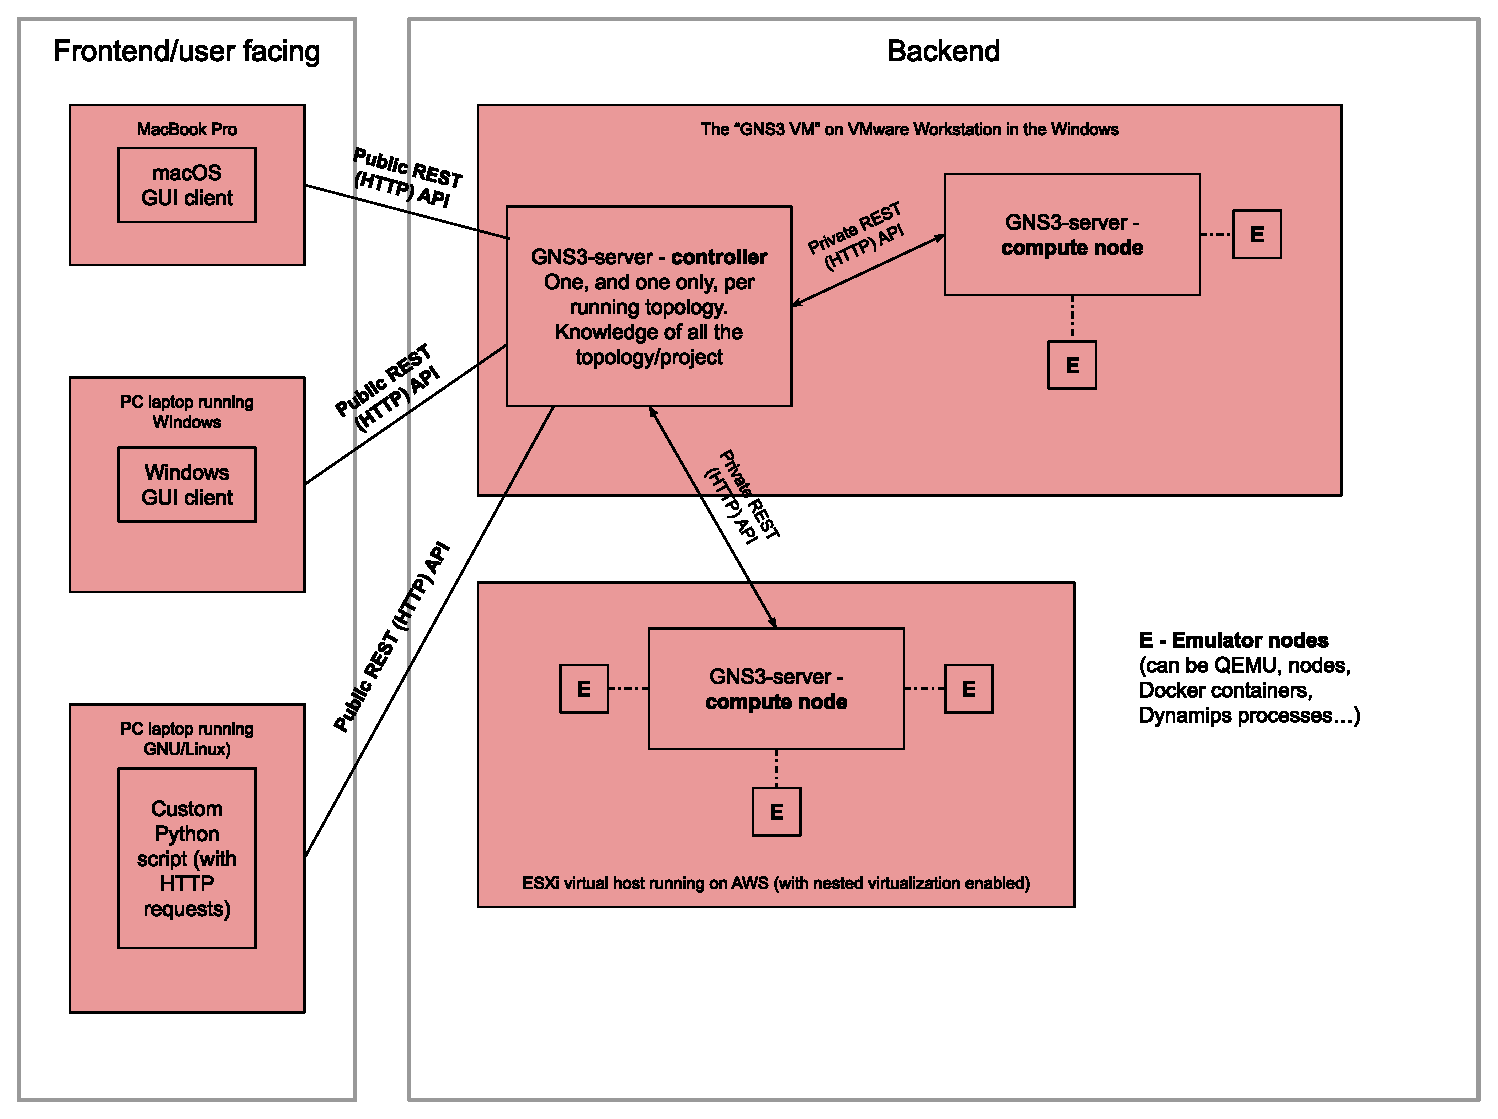
\includegraphics[width=1\textwidth]{gns3-running-arch}
  \caption{The GNS3 architecture}
  \label{fig:gns3-running-arch}
\end{figure}

In this section, an attempt is made to describe the different parts of GNS3 is to see what role they play in an execution of a topology (i.e. a project) and how they communicate with each other.
The diagram in figure~\ref{fig:gns3-running-arch} is based upon~\cite{ytgns3arch22}.
A central idea is the potentially distributed nature of the components, allowing for a complex topology with many nodes to be run across many hosts, dividing the computing power load across more than one host.
The precautions that must be taken to ensure a performance, and some caveats, will be explained in~\ref{sec:gns3inaction}. % TODO precautions taken?

The GNS3 server program, has two possible roles in a GNS3 session. % TODO define what's a "GNS3 session"
Those are: ``computes'' and the controller.
A GNS3 session only has one controller.
Any desktop installation of GNS3 comes with the server installed, able to run as the controller.
The GNS3 GUI will connect to the controller and allow for the user to ``open'' a topology on it.
The communication, as said, between any client (the GUI or any script) and the controller happens through HTTP requests following a REST approach. % TODO link acronyms et al to gls
The controller has knowledge of all the hosts running nodes of the topology.
Those nodes are run using ``computes'', which are processes of the GNS3 server whose responsibility is to expose a private REST API---\emph{not the same} as the one that the controller exposes and only to be used internally---to receive commands from the decision point (the controller) and locally interact with QEMU processes, Docker containers, Dynamips processes, or other emulation, container, or virtualization solution over which a node of the topology (an IOS Cisco router, a host, or a NAT node) is executed.

Therefore, on the diagram depicted in figure~\ref{fig:gns3-running-arch}, we see a topology running on distributed machines---these could be exclusively interconnected virtual machines on the same physical computer, without any loss of generality. % TODO put the background of the word of the same color that it has on the diagram
What matters is that they are running in hosts able to communicate with each other via IP and where GNS3 server is supported.
Each magenta rectangle is a separate host. % TODO check the color name
On the backend there are two hosts.
One of the hosts is the ``GNS3 VM'', running over VMware Workstation for Windows, and is ``playing'' both roles of the GNS3 server at the same time: it is the (single) controller for the running topology, which means that it loads the file describing the topology and has the receives the client's input, while knowing on which host should each topology node by run.
Then, it has a compute running alongside, to run two topology nodes.
These can be, for example, Cisco IOSv routers. % TODO how to spell IOSv. Somewhere we need to talk about this
On another host, which is a ESXi virtual machine (running on some infrastructure), \emph{with nested virtualization enabled}, the GNS3 server is also running, but there is no controller---all it does is ``blindly'' (at specific requests from the controller via the private REST API) perform, in the compute nodes, the necessary local interactions with the emulators. % TODO ESXi cite/link something
In the picture, there are three nodes running, which can be, for example, a Dynamips emulator for a <supported Dynamips Cisco router> and two hosts running on Docker. % TODO replce with a real model

% end of section gns3architecture
